\documentclass{article}

\usepackage{microtype}

\usepackage[T1]{fontenc}
\usepackage{mathpazo}
\usepackage{amsmath,amsthm}
\newtheorem{theorem}{Theorem}
\newtheorem{proposition}{Proposition}
\newtheorem{definition}{Definition}
\newtheorem{lemma}{Lemma}
\newtheorem{exercise}{Exercise}
\newtheorem{example}{Example}
\newtheorem{corollary}{Corollary}

\usepackage{algpseudocode}
\usepackage{listings}
\lstset{basicstyle=\ttfamily}

\usepackage{tcolorbox}
\newtcolorbox{examplebox}[1]{width=\textwidth,colback={lightgray},title={#1},colbacktitle={lightgray!50},coltitle={black}}
\newtcolorbox{algobox}[1]{width=\textwidth,colback={lightgray},title={#1},colbacktitle={lightgray!50},coltitle={black}}

\usepackage{tikz}
\usetikzlibrary{shapes,snakes,positioning,decorations.pathreplacing}

\usepackage{answers}
\Newassociation{sol}{Solution}{ans}
\Newassociation{hint}{Hint}{hints}



\title{Basic Arithmetic}
\author{Balagopal Komarath}

\begin{document}

\maketitle

\section{Decimal Notation}

\Opensolutionfile{ans}[ans1]

Imagine that you are putting apples into a box and you want to keep
track of how many apples you have placed in the box.  You decide to
use 10 distinct symbols $0, \ldots, 9$ to keep track of how many
apples you have put in the box. Each of these symbols model a
different state of the box of apples. The state $0$ corresponds to no
apples in the box. The state $1$ corresponds to the state reached by
placing one apple into the empty box and so on. If we are in state 4
and we throw in one more apple, then we reach state 5. This can be
written in math notation as $4 + 1 = 5$ (one added to four equals
five). This operation is called \emph{addition}. You can add any two
symbols. The sum $4 + 2$ corresponds to the state of the box after
you have put in four apples followed by two more apples. Indeed, this is
the same state as the one obtained by putting five apples followed by
a single apple. We therefore have the equality $4 + 2 = 5 +
1$. Infact, we have a symbol for this, namely $6$.

\subsection{Two digit numbers}
You place apples until you reach the state $9$. If you throw in one
more apple, then we know that this state should be $9 + 1$. Why?
Because, if we have placed four apples and then placed one more, then
the new state was denoted by $4 + 1$. So for consistency, if we have
already placed $9$ and then add one more, then the current state
should be $9 + 1$. We have no symbol to denote this state. Why?
Because, representing all states using distinct symbols would be
foolish. Imagine that you have very many apples; then you will require
as many symbols as the total number of apples. This is clearly not
feasible.

Now we are faced with a dilemma. We know that $9 + 1$ is a valid state
yet we do not have a ``clean'' representation for it. Let us
temporarily call $9 + 1 = x$ (as in we have placed $x$ apples). This
is a fundamental operation in math. Whenever we encounter an unknown,
we assign a placeholder symbol to it (the letter $x$ here) and try and
analyze the properties that the unknown should satisfy.

What is the state when we have placed 2 apples after we have placed 9?
The answer is that we are in state $9 + 2$. But, we know that this is
the same state that we will reach if we had placed one apple after
placing $x$, namely $x + 1$. Therefore, we have the equality
$9 + 2 = x + 1$ for our $x$. Continuing in this vein, we find that
there are numbers $x + 2, x + 3,\ldots, x + 9$ that correspond to
placing two apples after placing $x$ apples etc. What is the state
once we place one more apple after we have placed $x + 9$?  Obviously,
this number is $(x + 9) + 1$. The paranthesis around $x + 9$ indicate
that the sequence of operations is as follows: place $x$ apples, place
$9$ more, and then place one more. If we simply wrote $x + 9 + 1$,
then this could have been interpreted as the different sequence of
events: placing $x$ apples, then take a box that has $9+1$ apples, and
then move all the apples in this box to the box containing $x$
apples. This sequence is denoted by the symbols $x + (9 + 1)$.

\begin{center}
  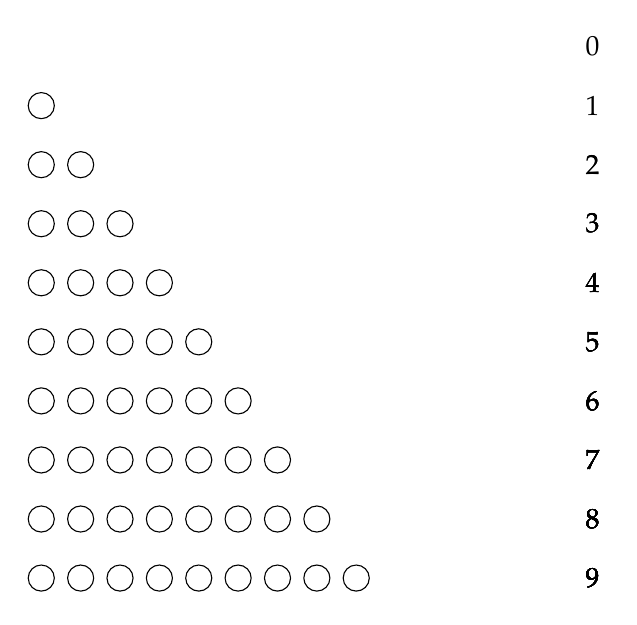
\begin{tikzpicture}
    \foreach \x in {0,...,8}
    {
      \pgfmathtruncatemacro{\xx}{8-\x}
      \foreach \y in {0,...,\xx}
      {
        \pgfmathtruncatemacro{\xlabel}{
          \xx+1
        }
        \node [circle,draw] at (0.5*\y,0.75*\x) {};
        \node at (7,0.75*\x) {$\xlabel$};
      }
    }
    \node at (7,0.75*9) {$0$};
  \end{tikzpicture}
\end{center}

A little bit of thought should reveal that the both sequences of
events described above lead to the same state. i.e.,
$(x + 9) + 1 = x + (9 + 1)$ and therefore we can simply write
$x + 9 + 1$.  We had already named $9 + 1$ as $x$. Therefore,
$x + 9 + 1 = x + x$. i.e., this is equivalent to placing $x$ apples
followed by placing $x$ more apples. The state $x + x$ is written as
$2x$ (read two times x).

(Associativity of Addition) For any three numbers $a$, $b$, and $c$,
we have $(a+b)+c = a+(b+c)$.

\begin{exercise}
  What is a natural notation for the state reached by placing $x$,
  $x$, 9, and then one more apple in the box?
  \begin{sol}
    $3x$ (Read ``three times x'').
  \end{sol}
\end{exercise}

There is nothing special about the number $2$ in the number $2x$. The
numbers $3x$, $4x$ etc. are all equally valid. Indeed, $3x$
corresponds to placing $x$ apples three times (or equivalently, you
can think of this as placing three bags each containing $x$
apples). What is the number $1x$? It is placing $x$ apples a single
time, or in other words, placing $x$ apples. But, this is the same as
the number $x$. Therefore, we have $1x = x$. What is $0x$? This is
placing $x$ apples zero times, or in other words, we aren't placing
any apples. This is just the number $0$. Therefore, we have $0x =
0$. There is nothing special about the number $x$ in the notation $2x$
too. The number $2.3$ is equally valid. It is placing $3$ apples two
times, or the number $6$. This operation is called
\emph{multiplication}. For any two numbers $a$ and $b$, the number
$a.b$ (read $a$ times $b$) corresponds to the total number of apples
in $a$ boxes where each box contains $b$ apples. Pictorially, we can
represent this as apples arranged in a rectangle of $a$ rows where
each row contains $b$ apples.

\begin{center}
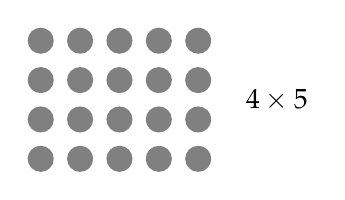
\begin{tikzpicture}
  \foreach \x in {0,...,4}
  \foreach \y in {0,...,3}
  \node [fill=gray,circle] at (0.5*\x,0.5*\y) {};
  \node at (3,0.75) {$4\times 5$};
\end{tikzpicture}
\end{center}

\subsection{Arbitrary number of digits}
Assume that you have placed $9x + 9$ apples and then you placed one
more. The new state is $9x + 9 + 1 = 9x + x$. This is the same state
as reached by placing $9x$ apples and then $x$ more. If you think
about this, this is the same state that you will reach if you place
$x$ apples in the box and repeat it $x$ times (If you do something $9$
times and then do it one more time you have done it $x$ times by
definition of $x$). When we placed $x$ apples two times, we wrote
$2x$. Therefore, when we place $x$ apples $x$ times, we shall write
$x.x$. This number is denoted by $x^2$ (read x squared). Note that
there is nothing special about $x$ in this notation. The notation
$2^2$ with $2$ substitued for $x$ is also a valid number. Just because
we have named it $x$ doesn't make it special in any way. Now what is
$2^2$? It is placing $2$ apples $2$ times. But we already have a
symbol associated with that state, namely $4$. So we don't write $2^2$
usually, we simply write $4$.

The number $x^2$ can also be represented as $x^2 + 0x + 0$. i.e., put
$x^2$ apples, then put $x$ apples zero times (if you do anything zero
times, then you are not doing it at all, $0x = 0$), then put zero more
apples into the box (i.e., no apples).

We have now derived the decimal notation. The number $x^2$ a.k.a
$\mathbf{1}x^2 + \mathbf{0}x + \mathbf{0}$ is usually written
$\mathbf{100}$. Here $1x^2 = x^2$, just like $1x = x$. In fact, $1.a =
a$ for any number $a$ and not just $x$ and $x^2$. Why? Because if you
place $a$ apples one time, then you have placed $a$ apples.

(Decimal form) Any of the numbers $0,\dotsc,9$ is a single digit
number. Any number that can be expressed as $ax + b$, where $a$ and
$b$ are single digit numbers is a two-digit number and written as $ab$
in decimal form. For example, $2x + 3 = 23$. Similarly, any number
that can be expressed as $ax^2+bx+c$ where $a$, $b$, and $c$ are
single digit numbers is a three-digit number and so on.

The decimal notation is nothing but dropping the $x$'s from our
representation. We will drop the $x$'s from here on and use decimal
notation whenever it is convenient. It is understood that, for
example, $123$ is the number $1x^2 + 2x + 3$ where $x = 9 + 1$.


\begin{exercise}
  What is the decimal form of the number $9x^2 + 9x + 9 + 1$?
  \begin{sol}
    $9x^2 + 9x + x = 9x^2 + x^2 = x.x^2 = x^3 = 1000$
  \end{sol}
\end{exercise}  

\section{Addition}

We have the set of numbers $0, 1, \ldots, 9, \ldots ,100, \ldots$
called the \emph{natural numbers}. How can we add two natural numbers?
We know how to add single digit numbers. For example, $3 + 4 = 7$, $5
+ 5 = 9 + 1 = 10$ and so on. We should be able to add any two natural
numbers.

\begin{center}
  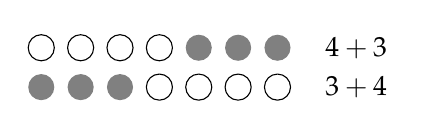
\begin{tikzpicture}
    \node [circle,fill=gray] at (0, 0) {};
    \node [circle,fill=gray] at (0.5, 0) {};
    \node [circle,fill=gray] at (1, 0)  {};
    \node [circle,draw] at (1.5, 0)  {};
    \node [circle,draw] at (2, 0)  {};
    \node [circle,draw] at (2.5, 0)  {};
    \node [circle,draw] at (3, 0)  {};
    \node at (4, 0) {$3+4$};
    
    \node [circle,draw] at (0, 0.5)  {};
    \node [circle,draw] at (0.5, 0.5)  {};
    \node [circle,draw] at (1, 0.5)  {};
    \node [circle,draw] at (1.5, 0.5)  {};
    \node [circle,fill=gray] at (2, 0.5) {};
    \node [circle,fill=gray] at (2.5, 0.5)  {};
    \node [circle,fill=gray] at (3, 0.5)  {};
    \node at (4, 0.5) {$4+3$};
  \end{tikzpicture}
\end{center}


Let us try and add 19 to 25. We can write $19 = x + 9$ and
$25 = 2x + 5$. Now, $25 + 19 = 2x + 5 + x + 9$. Any two numbers $a$
and $b$ satisfy the property $a+b = b+a$ called the commutativity of
addition. Since we can add numbers in any order by this property let's
add 9 to 5 first. We know that $9 + 5 = x + 4$. Here, we added two
single digit numbers and got a two digit number. The $x$ in this sum
is called the \emph{carry}. Now if we add together the remaining two
parts $2x$ and $x$, we will get $3x$. So the result is $3x + x +
4$. We can write $3x + x$ as $4x$. The $x$ that was generated when
adding $9$ to $5$ in the first step was \emph{carried over} to the
higher digit. This is why it's called a carry. The final answer is
$4x + 4 = 44$. In decimal notation, one can do this summation as
follows:

\vskip2ex

\vbox{
  \hbox{$\overset{1}{2}$5 +}
  \hbox{\underline{19}}
  \hbox{44}
}

Let us try doing a more complicated sum. We will add $876$ to
$579$. We know that $579 = 5x^2 + 7x + 9$ and $876 = 8x^2 + 7x +
6$. As we did in the previous some, we will group terms by $x$ and do
the sum. We write $876 + 579 = (5x^2 + 8x^2) + (7x + 7x) + (9 + 6)$
(associativity and commutativity of addition enables this). Now, we
know $9 + 6 = x + 5$ (Note the carry) and
$7x + 7x = 9x + 5x = 9x + x + 4x = x^2 + 4x$ . Now,
$x^2+4x+x+5=x^2+5x+5$. The $x^2$ in this sum is a carry generated by
adding up $x$ terms and the lower terms. Adding up the $x^2$ terms we
get, $5x^2 + 8x^2 = 9x^2 + 4x^2 = 9x^2 + x^2 + 3x^2 = x^3 +
3x^2$. Finally, $x^3+3x^2+x^2+5x+5 = x^3+4x^2+5x+5 = 1455$.  Again,
the $x^3$ obtained by adding $x^2$ terms and lower terms is a
carry. The decimal notation lends itself to expressing these
calculations easily as shown below. From here on, we will calculate
all sums using decimal notation.

\vskip2ex

\vbox{
  \hbox{$\overset{1}{\phantom{0}}\overset{1}{8}\overset{1}{7}6$ +}
  \hbox{\phantom{0}\underline{579}}
  \hbox{1455}
}

\begin{center}
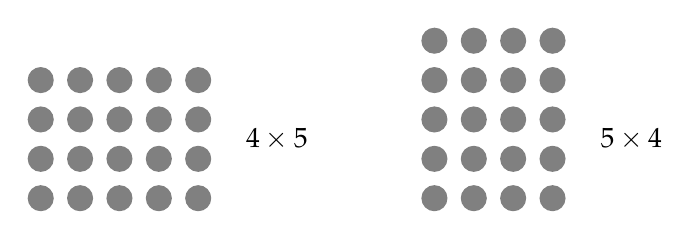
\begin{tikzpicture}
  \foreach \x in {0,...,4}
  \foreach \y in {0,...,3}
  \node [fill=gray,circle] at (0.5*\x,0.5*\y) {};
  \node at (3,0.75) {$4\times 5$};
  
  \foreach \x in {0,...,3}
  \foreach \y in {0,...,4}
  \node [fill=gray,circle] at (5+0.5*\x,0.5*\y) {};
  \node at (5+0.5*5,0.75) {$5\times 4$};

\end{tikzpicture}
\end{center}

(Distributivity of Multiplication over Addition) For any $a$, $b$, and
$c$, we have $(a+b)c = ac + bc$.

\begin{center}
  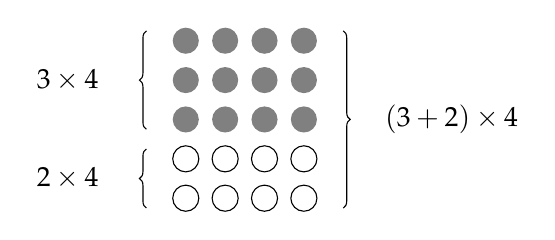
\begin{tikzpicture}
    \foreach \a in {0,...,1}
    \foreach \c in {0,...,3}
    \node [circle,draw] at (0.5*\c, 0.5*\a) {};
    \draw [decorate,decoration=brace] (-0.5, -0.125) -- (-0.5, 0.625) node [black,midway,xshift=-1cm] {$2\times 4$};
    
    \foreach \b in {0,...,2}
    \foreach \c in {0,...,3}
    \node [circle,fill=gray] at (0.5*\c,1+0.5*\b) {};
    \draw [decorate,decoration=brace] (-0.5, 0.875) -- (-0.5, 2.125)  node [black,midway,xshift=-1cm] {$3\times 4$};;

    \draw [decorate,decoration={brace,mirror}] (2, -0.125) -- (2, 2.125)  node [black,midway,xshift=1.375cm] {$(3+2)\times 4$};;
  \end{tikzpicture}
\end{center}

Using distributivity could make adding terms with the same power of
$x$ such as $7x+7x$ easier. For example,
$7x+7x = (7+7)x = (x+4)x = x^2+4x$.

\Closesolutionfile{ans}
\section*{Answers}
\input{ans1}
\end{document}
